% Report in the ACM sigconf format (same layout as the DataLab 1 report).
% `nonacm` removes the ACM copyright block, conference footer and reference format line.
% `balance=false` fills the left column of the last page before the right one.
% Page budget (A2 instructions): at most 5 pages of content; the supplementary material follows.
\documentclass[sigconf,nonacm,balance=false]{acmart}

\usepackage{booktabs}
\usepackage{multirow}
\usepackage{float}     % [H] floats in the supplementary material
\usepackage{titletoc}  % partial table of contents of the supplementary material
\setlength{\textfloatsep}{8pt plus 2pt minus 2pt}
\setlength{\dbltextfloatsep}{8pt plus 2pt minus 2pt}

% Notation shared by all sections.
\newcommand{\finc}{FID$_\mathrm{Inc}$}
\newcommand{\fcnn}{FID$_\mathrm{CNN}$}

\settopmatter{printacmref=false, printfolios=true}

\begin{document}

\title{Data, Training and Inference Levers for a Fixed-Architecture GAN}
\subtitle{What helps a small MNIST generator, and why}

\author{Nicod\`eme Gorge}
\affiliation{%
  \institution{PSL University, Master IASD}
  \city{Paris}
  \country{France}}
\author{No\'e Mosca}
\affiliation{%
  \institution{PSL University, Master IASD}
  \city{Paris}
  \country{France}}
\author{Quentin Revillon}
\affiliation{%
  \institution{PSL University, Master IASD}
  \city{Paris}
  \country{France}}
\renewcommand{\shortauthors}{}

\begin{abstract}
We study a GAN whose generator architecture is imposed: a small fully connected network that maps 100 random numbers to a $28\times28$ MNIST digit. Since its capacity is fixed, we act on the three remaining levers: the training data, the training procedure, and the way images are drawn at inference. Each change is tested against the same baseline, with three seeds, a common budget of 100,000 updates and the Inception FID of the course platform (38.7 for the baseline). Neither data lever helps: keeping only the most typical images trades recall for little precision, and instance noise changes neither the score nor the collapse rate. The training lever gives most of the gain, but only as a combination: a relativistic loss with an R1 penalty balances the ten digits without changing the FID, an exponential moving average (EMA) of the generator alone reaches 30.0, and both together reach 22.1. Discriminator rejection sampling improves the baseline but not this model, whose discriminator barely separates real from generated images (AUC 0.57); refitting its last layer restores the gain (19.7). The submitted model scores 19.4 on the MNIST test set. We also show that a FID computed on a digit classifier mainly measures digit balance, which is why we rank models with the Inception FID.
\end{abstract}


\keywords{generative adversarial networks, MNIST, relativistic loss, weight averaging, rejection sampling, FID}

\maketitle

\section{Introduction}
A generative adversarial network trains a generator $G$, which maps a random vector $z$ to an image, against a discriminator $D$, which learns to tell real images from generated ones \cite{goodfellow2014}. In this assignment the architecture of $G$ is imposed: a four-layer fully connected network from 100 inputs to 784 pixels. Recent GAN recipes owe much of their progress to larger and convolutional generators \cite{huang2024}; here that option is closed. We therefore ask which of the three remaining levers improves a small, fixed generator: what it sees (\emph{data}), how it is trained (\emph{training}), and how images are drawn once it is trained (\emph{inference}).

Each lever was studied by one member of the group on a separate branch, then all were brought onto one protocol so that their effects can be compared and combined. GAN results vary strongly between seeds, so every variant is trained with three seeds and compared with $t$-tests; with three seeds, only differences of about 3.6 FID points are reliably detectable.

\paragraph{Contributions}
(1) A study of which score to trust: a FID on a digit classifier mostly measures digit balance, while the Inception FID measures stroke quality (Section~\ref{sec:fid}).
(2) Two data levers, instance selection and instance noise, and why neither transfers to MNIST (Section~\ref{sec:data}).
(3) A loss $\times$ EMA ablation showing that a relativistic loss with R1 and weight averaging only pay off together (Section~\ref{sec:training}).
(4) An analysis of why discriminator rejection sampling fails on a well-trained GAN and how recalibrating $D$ fixes it (Section~\ref{sec:inference}).
(5) The combined pipeline and the submitted model (Section~\ref{sec:combination}).

\section{Related Work}
\paragraph{Data}
Instance selection removes the least typical training images, scored by a density model in the feature space of a pretrained network, so that a GAN of limited capacity spends it on dense regions; on ImageNet it improves the FID of conditional generators \cite{devries2020}. Instance noise adds Gaussian noise to both real and generated inputs of $D$ so that the two distributions overlap and $D$ cannot win too early \cite{sonderby2017,arjovsky2017}.

\paragraph{Training}
The relativistic loss asks $D$ whether a real image is more realistic than a generated one rather than judging each image alone \cite{jolicoeur2019}. The zero-centred R1 penalty on real images makes GAN training locally convergent \cite{mescheder2018}. R3GAN combines both, with an R2 penalty on generated images, into a modern baseline \cite{huang2024}. Averaging the generator's weights over iterations (EMA) is a cheap and widely used improvement \cite{yazici2019}.

\paragraph{Inference}
Discriminator rejection sampling (DRS) keeps each generated image with a probability derived from $D$'s score, which corrects $G$ if $D$ estimates the density ratio well \cite{azadi2019}. Optimal budgeted rejection sampling (OBRS) is the optimal acceptance rule for a fixed number of proposals per kept image \cite{verine2024}.

\paragraph{Evaluation}
The FID compares Gaussian fits of Inception features \cite{heusel2017,szegedy2016}; its sensitivity to ImageNet classes \cite{kynkaanniemi2023} and to missing modes \cite{lucic2018} has been questioned, and domain-specific feature extractors are sometimes used on MNIST \cite{binkowski2018}. Precision and recall measure quality and coverage with $k$-nearest-neighbour manifolds \cite{kynkaanniemi2019}.

\section{Experimental Setup}
\label{sec:setup}
\paragraph{Data and model}
We use MNIST \cite{lecun1998}, split once and for all: 50,000 training images, 10,000 validation images taken from the original training set (fixed permutation), and the 10,000 test images, used only for the numbers reported here. Pixels are scaled to $[-1,1]$. $G$ (100--256--512--1024--784) and $D$ (784--1024--512--256--1) are the provided fully connected networks, with about 1.5M parameters each; $D$ ends with a sigmoid, and its pre-sigmoid output is its \emph{score}.

\paragraph{Common protocol}
All variants use the provided optimizer (Adam, learning rate $2\cdot10^{-4}$, batch size 100) and the same budget of 200 epochs, i.e.\ 100,000 updates. We evaluate the last checkpoint, without choosing an epoch, and train three seeds per variant. The data-lever runs (Section~\ref{sec:data}) were trained earlier on a slightly different protocol (all 60,000 images, 120,000 updates, no EMA) and are compared only with their own reference.

\paragraph{Metrics}
Each model draws 10,000 images, compared with the 10,000 test images. The main score is the platform's \finc{}, computed on the 2,048 pool features of Inception-v3 \cite{szegedy2016} (lower is better). Precision and recall use VGG-16 features \cite{simonyan2015} and $k=5$ on 9,984 images, as on the platform. We also compute \fcnn{}, the same formula on the features of a small MNIST classifier trained by the group (98.7\% test accuracy); it costs seconds instead of minutes, so we used it during training. Real against real images gives the floor of each score: 1.5 for \finc{} and 2.7 for \fcnn{}. A run is \emph{collapsed} when its classifier-based recall falls below 0.01.

\paragraph{Hardware}
Runs were trained on an NVIDIA A100 (Juliet cluster) or on an Apple M3 (MPS). Both give bit-identical weights for a given configuration on the same machine, but not across machines: the same baseline scores 36.6 on the cluster and 38.7 on the laptop. Effects of an add-on (EMA, rejection) are therefore always measured on the same runs.

\section{Methods}
\label{sec:method}
\paragraph{Instance selection}
For each digit, we fit a Gaussian to the classifier features of its training images and keep the 95, 90, 75 or 50\% of images with the highest log-likelihood, following \cite{devries2020}. The GAN only sees this subset; evaluation is still made against all test images.

\paragraph{Instance noise}
Every input of $D$, real or generated, receives Gaussian noise of standard deviation $\sigma_t$, annealed linearly from $\sigma_0$ to 0 over the first 100 epochs \cite{sonderby2017}; we test $\sigma_0\in\{0.1,0.3\}$. $G$ and the saved images are not noised.

\paragraph{Relativistic loss with R1 (RpGAN + R1)}
With $f$ the score of $D$, $x$ a real image, $\tilde x=G(z)$ and $\mathrm{sp}(t)=\log(1+e^t)$:
\begin{align*}
L_D &= \mathbb{E}\big[\mathrm{sp}\big(f(\tilde x)-f(x)\big)\big] + \tfrac{\gamma}{2}\,\mathbb{E}\big[\|\nabla_x f(x)\|^2\big],\\
L_G &= \mathbb{E}\big[\mathrm{sp}\big(f(x)-f(\tilde x)\big)\big].
\end{align*}
This is R3GAN \cite{huang2024} without the R2 term, which gave no measurable gain in our preliminary runs. A sweep over $\gamma\in\{0.1,1,10\}$ with three seeds each (100 epochs) gave: all runs diverge at 0.1, $\gamma=1$ is best, $\gamma=10$ learns more slowly. We keep $\gamma=1$; the penalty adds about 5\% to the training time.

\paragraph{Exponential moving average (EMA)}
After each update, $G_\mathrm{EMA}\leftarrow 0.999\,G_\mathrm{EMA}+0.001\,G$, i.e.\ an average over roughly the last two epochs \cite{yazici2019}. $G_\mathrm{EMA}$ is used for evaluation and saved as the delivered generator; the raw $G$ is saved too, so both can be compared on the same run.

\paragraph{Rejection sampling}
DRS \cite{azadi2019} keeps a proposal with probability $\sigma(\hat F)$, where $\hat F = f - f_M - \log(1-e^{f-f_M-\epsilon}) - \gamma'$, $f_M$ is the highest score seen and $\gamma'$ is set per batch to the 80th percentile of $\hat F$ ($\epsilon=10^{-6}$). OBRS \cite{verine2024} uses a budget of $K=3$ proposals per kept image. Both need a score close to $\log p_\mathrm{data}/p_G$. \emph{Recalibration}, as in \cite{azadi2019}, keeps $D$'s hidden layers and refits its last layer as a logistic regression on 10,000 real validation images against 10,000 generated ones; the recalibrated $D$ has the same architecture as the original one.

\section{Results}

\begin{figure*}[t]
  \centering
  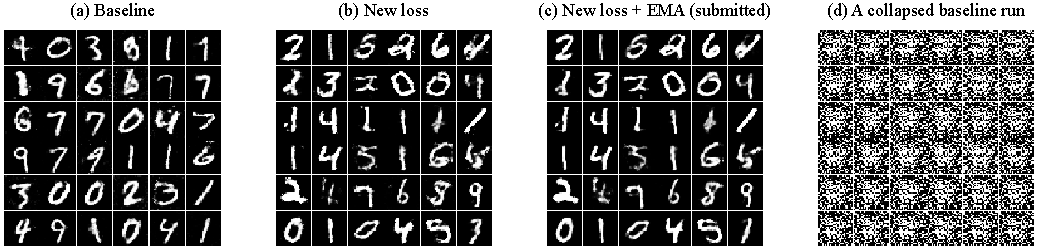
\includegraphics[width=\textwidth]{figs/combination_samples.pdf}
  \caption{Samples from the same 36 latent vectors $z$. (a) Baseline: readable digits, but many ``1''s and ``7''s and few ``2''s. (b) RpGAN + R1, raw generator: all digits appear. (c) Same run, averaged generator: cleaner strokes (submitted generator). (d) A collapsed baseline run.}
  \Description{Four grids of 6 by 6 generated digits. The baseline grid contains many ones and sevens; the RpGAN grids contain all ten digits, with smoother strokes for the averaged generator; the collapsed run outputs identical noise patterns.}
  \label{fig:samples}
\end{figure*}

\subsection{Which score should we trust?}
\label{sec:fid}
Changing the loss divides \fcnn{} by nine but leaves \finc{} unchanged (Table~\ref{tab:results}), so the two scores must see different defects. To find out which, we degraded \emph{real} test images in controlled ways (Figure~\ref{fig:fid}). \fcnn{} reacts to the balance between digits: removing one digit raises it from 2.7 to 40, and giving real images the baseline's digit proportions raises it to 124, close to the baseline's 162. \finc{} barely moves (2.4 and 7.4, for a baseline at 40). Conversely, noise on a quarter of the images is enough for \finc{} to reach the baseline's score (41) while \fcnn{} stays at 18. Digit identity explains 67\% of the variance of the classifier's features against 26\% for Inception's, in line with \cite{kynkaanniemi2023}. A direct check confirms it: resampling the baseline's images so that every digit is equally frequent lowers \fcnn{} from 162 to 32 but \emph{raises} \finc{} from 39.9 to 46.2, because the added rare digits are badly drawn.

We therefore rank models with \finc{}, which is also the platform's score and varies less between seeds (3--6\% of its value against 11--25\% for \fcnn{}), and keep \fcnn{} with the histogram of predicted digits as a diagnostic of digit balance. To see the quality of each digit, we also compute a per-digit \finc{}: our classifier sorts the generated images by digit, and 1,000 images of each digit are compared with real images of the same digit.

\begin{figure}[t]
  \centering
  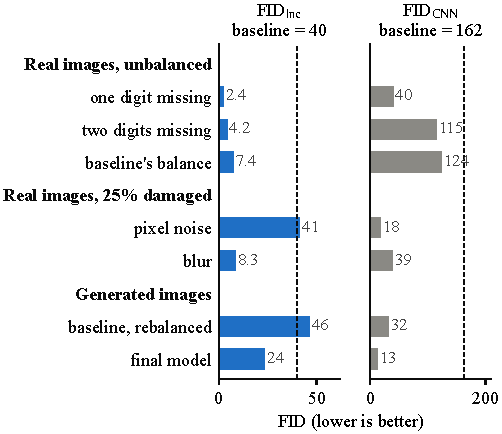
\includegraphics[width=0.82\columnwidth]{figs/fid_sensitivity.pdf}
  \caption{Both FIDs on deliberately damaged \emph{real} test images (10,000 images). Dashed lines: scores of the baseline GAN. Undamaged real images score 1.5 (\finc{}) and 2.7 (\fcnn{}).}
  \Description{Two horizontal bar charts. Missing digits and the baseline's digit balance give large FID-CNN values but small Inception FID values; pixel noise on a quarter of the images gives an Inception FID of 41, as high as the baseline, but a small FID-CNN.}
  \label{fig:fid}
\end{figure}

\subsection{Data lever}
\label{sec:data}
% Sources: data/nico_data_test.csv (selection, data protocol, runs with classifier recall >= 0.01),
% data/juliet2_test.csv (baseline loss + EMA +- noise 0.3), data/comparison_local.csv (RpGAN + R1 + EMA +- noise 0.3).
\begin{table}[t]
\centering
\small
\setlength{\tabcolsep}{4pt}
\caption{Data lever: \finc{} (mean $\pm$ s.d.\ over non-collapsed runs), precision and recall. Collapsed runs are counted separately.}
\label{tab:data}
\begin{tabular}{lcccc}
\toprule
Variant & Collapsed & \finc{} & Prec. & Rec.\\
\midrule
\multicolumn{5}{l}{\emph{Instance selection (data protocol, no EMA)}}\\
All images (reference) & 3/8 & $35.4\pm0.9$ & 0.51 & 0.52\\
Keep 95\% & 2/5 & $38.2\pm2.7$ & 0.49 & 0.48\\
Keep 90\% & 2/5 & $35.8\pm3.3$ & 0.53 & 0.49\\
Keep 75\% & 0/3 & $40.8\pm3.9$ & 0.54 & 0.40\\
Keep 50\% & 4/8 & $47.8\pm2.9$ & \textbf{0.56} & 0.32\\
\midrule
\multicolumn{5}{l}{\emph{Instance noise $\sigma_0=0.3$ (common protocol, EMA)}}\\
Baseline loss & 0/3 & $30.0\pm0.2$ & 0.56 & 0.54\\
\quad + noise & 2/5 & $30.1\pm1.3$ & 0.56 & 0.54\\
RpGAN + R1 & 0/3 & $22.1\pm1.3$ & 0.59 & 0.59\\
\quad + noise & 0/3 & $21.4\pm0.6$ & \textbf{0.60} & \textbf{0.61}\\
\bottomrule
\end{tabular}
\end{table}

\paragraph{Instance selection}
No selection rate beats the reference (Table~\ref{tab:data}): keeping 90\% ties (35.8 against 35.4) and keeping 50\% is clearly worse (47.8). Precision rises from 0.51 to 0.56 but recall falls from 0.52 to 0.32: the generator draws fewer odd digits, but also fewer kinds of digits. At 50\% it no longer draws any ``0'', which is 10\% of the data. The same trade-off appears with VGG and with classifier features, so it is not an artefact of selecting and evaluating with the same classifier.

\paragraph{Instance noise}
Noise does not change \finc{} with either loss ($p=0.91$ and $p=0.46$). Nor does it prevent collapses: with the baseline loss, 2 of 5 noised runs collapsed on the common protocol, and a paired rerun of 8 seeds on the data protocol gave 1 collapse out of 8 with noise against 3 out of 8 without ($p=0.57$). In 17 of the 19 collapsed runs we inspected, $D$ gives generated images a probability below $10^{-12}$ of being real; the binary cross-entropy of the provided code then clips, $G$'s gradient vanishes and $G$ stops learning. Noise spread over all pixels does not remove the few directions that separate real from generated images, so it cannot prevent this.

\subsection{Training lever}
\label{sec:training}
% Sources: data/juliet2_test.csv (baseline loss, raw G and G_EMA of the same runs, A100),
% data/comparison_local.csv + data/juliet2_test.csv (RpGAN + R1: G_EMA and raw G of the same runs, M3),
% data/ema_summary.csv. p-values: paired t-tests over the 3 seeds (EMA rows), Welch test (loss row).
\begin{table}[t]
\centering
\small
\setlength{\tabcolsep}{6pt}
\caption{Loss $\times$ EMA, \finc{} on the common protocol (3 seeds). Each EMA effect compares the raw and averaged generators of the same runs.}
\label{tab:loss-ema}
\begin{tabular}{lcc}
\toprule
 & Baseline loss & RpGAN + R1\\
\midrule
Raw generator & $36.6\pm1.3$ & $37.7\pm1.0$\\
Averaged generator (EMA) & $30.0\pm0.2$ & $\mathbf{22.1\pm1.3}$\\
\midrule
Effect of the EMA & $-6.7$ ($p=0.01$) & $-15.6$ ($p<0.001$)\\
\bottomrule
\end{tabular}
\end{table}

Table~\ref{tab:loss-ema} isolates the two ingredients. The new loss alone does not change \finc{} (37.7 against 36.6--38.7 for the baseline, depending on the machine). The EMA alone improves the baseline from 36.6 to 30.0. Together, they reach 22.1: the EMA gains more than twice as much with the relativistic loss as with the original one ($-15.6$ against $-6.7$, $p=0.002$), and the loss improves \finc{} by 8 points once the generator is averaged ($p=0.007$).

Figure~\ref{fig:perdigit} shows what each ingredient does. The relativistic loss \emph{rebalances the digits}: the baseline draws a ``1'' in a quarter of its images and a ``2'' in fewer than 2\%, whereas RpGAN + R1 draws each digit 8--12\% of the time. It also draws hard digits better, at fixed digit: the mean per-digit \finc{} drops from 63.6 to 55.4 ($p=0.005$), and that of ``2'' from 113 to 80. The global \finc{} hides these gains because the baseline's worst digits are also its rarest, so they weigh little in its score. No RpGAN + R1 run collapsed. The EMA then \emph{cleans the strokes of every digit} (mean per-digit \finc{} 37.3, Figure~\ref{fig:samples}c), which the global score does see.

\begin{figure}[t]
  \centering
  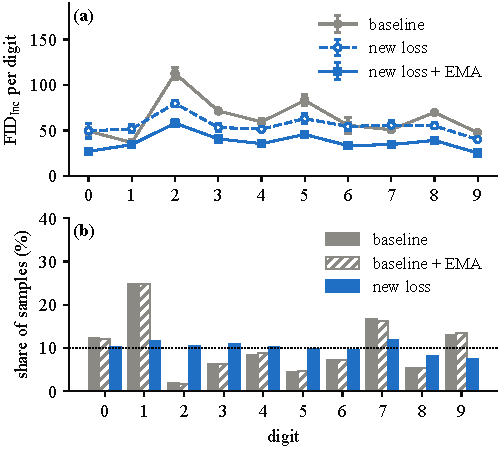
\includegraphics[width=0.86\columnwidth]{figs/training_perdigit.pdf}
  \caption{(a) Per-digit \finc{} (generated images of one digit against real images of the same digit; real data: 6.5--10.4). (b) Share of each digit among 10,000 samples; the dotted line is the balance of real data.}
  \Description{Top: per-digit FID; the baseline peaks at 113 on digit 2, the new loss lowers most digits and the averaged generator is lowest everywhere. Bottom: the baseline and baseline with EMA draw 25 percent ones and under 2 percent twos; the new loss is close to 10 percent for every digit.}
  \label{fig:perdigit}
\end{figure}

% Sources: data/comparison_local.csv (M3: baseline, RpGAN + R1 + EMA +- noise, +- DRS; one draw per seed),
% data/juliet2_test.csv (A100: baseline + EMA +- DRS, raw RpGAN + R1), data/drs_recalib_test.csv (recalibrated OBRS,
% 3 seeds x 2 draws). Submitted model: one run, platform evaluator on the MNIST test set.
\begin{table*}[t]
\centering
\small
\setlength{\tabcolsep}{5pt}
\caption{All configurations on the common protocol (200 epochs on 50,000 images, last checkpoint, 10,000 images against the MNIST test set), mean $\pm$ s.d.\ over 3 seeds. D, T, I: data, training and inference levers used. Precision and recall use VGG-16 features ($k=5$).}
\label{tab:results}
\begin{tabular}{lccccccccc}
\toprule
Configuration & D & T & I & \finc{}\,$\downarrow$ & Precision\,$\uparrow$ & Recall\,$\uparrow$ & \fcnn{}\,$\downarrow$ & Kept & Machine\\
\midrule
Baseline (provided loss) & & & & $38.7\pm1.2$ & 0.47 & 0.51 & 182 & 100\% & M3\\
\quad + DRS & & & \checkmark & $34.4\pm0.7$ & 0.51 & 0.49 & 154 & 30\% & M3\\
Baseline + EMA & & \checkmark & & $30.0\pm0.2$ & 0.56 & 0.54 & 182 & 100\% & A100\\
\quad + DRS & & \checkmark & \checkmark & $24.8\pm1.0$ & \textbf{0.62} & 0.53 & 167 & 31\% & A100\\
\midrule
RpGAN + R1, raw generator & & \checkmark & & $37.7\pm1.0$ & 0.47 & 0.47 & 19.7 & 100\% & M3\\
RpGAN + R1 + EMA & & \checkmark & & $22.1\pm1.3$ & 0.59 & 0.59 & 9.9 & 100\% & M3\\
\quad + instance noise $\sigma_0=0.3$ & \checkmark & \checkmark & & $21.4\pm0.6$ & 0.60 & \textbf{0.61} & \textbf{9.0} & 100\% & M3\\
\quad + DRS & & \checkmark & \checkmark & $22.0\pm1.1$ & 0.59 & 0.58 & 14.2 & 43\% & M3\\
\quad + OBRS, recalibrated $D$ & & \checkmark & \checkmark & $\mathbf{19.7\pm0.8}$ & \textbf{0.62} & 0.59 & 10.2 & 33\% & M3\\
\midrule
\textbf{Submitted}: RpGAN + R1 + EMA (seed 1), OBRS, recalibrated $D$ & & \checkmark & \checkmark & \textbf{19.4} & 0.61 & 0.60 & -- & 33\% & M3\\
\bottomrule
\end{tabular}
\end{table*}

\subsection{Inference lever}
\label{sec:inference}
% Source: data/drs_recalib_test.csv (A100; 3 seeds x 2 draws of 10,000 kept images each).
% Time: generation of 10,000 kept images on one A100, recalibration excluded (fitted once).
\begin{table}[t]
\centering
\small
\setlength{\tabcolsep}{3.2pt}
\caption{Rejection sampling with $D$ (3 seeds $\times$ 2 draws). AUC: probability that $D$ scores a real image above a generated one.}
\label{tab:rejection}
\begin{tabular}{lccccc}
\toprule
Filter & AUC & Kept & \finc{} & \fcnn{} & Time\\
\midrule
\multicolumn{6}{l}{\emph{Baseline}}\\
none & -- & 100\% & $38.7\pm0.8$ & 183 & 0.03\,s\\
DRS & 0.75 & 30\% & $34.3\pm0.7$ & 154 & 0.14\,s\\
OBRS & 0.75 & 33\% & $\mathbf{33.8\pm0.9}$ & 145 & 0.17\,s\\
OBRS, recalibrated & 0.83 & 33\% & $36.1\pm0.9$ & 83 & 0.16\,s\\
\midrule
\multicolumn{6}{l}{\emph{RpGAN + R1 + EMA}}\\
none & -- & 100\% & $22.0\pm1.3$ & 9.9 & 0.02\,s\\
DRS & 0.57 & 42\% & $22.1\pm1.0$ & 14.4 & 0.07\,s\\
DRS, recalibrated & 0.77 & 32\% & $20.2\pm1.1$ & 10.0 & 0.09\,s\\
OBRS, recalibrated & 0.77 & 33\% & $\mathbf{19.7\pm0.8}$ & 10.2 & 0.16\,s\\
\bottomrule
\end{tabular}
\end{table}

On the baseline, filtering works with $D$ as trained: DRS improves \finc{} from 38.7 to 34.3 and OBRS to 33.8 (Table~\ref{tab:rejection}); on the averaged baseline, DRS goes from 30.0 to 24.8. On the final model, it does nothing to \finc{} (22.0 to 22.1) and worsens \fcnn{} on every seed (9.9 to 14.4). The reason is that this $D$ can barely tell real from generated images: its AUC is 0.57, against 0.75 for the baseline's. A filter based on such a score keeps images almost at random (42\% instead of the intended 30\%), and the slight preferences it has shift the digit balance, which only \fcnn{} sees. Part of this comes from $D$ never having seen the averaged generator, but DRS also fails on the raw generator (37.7 to 38.0), so it is not the whole story.

Recalibrating $D$'s last layer raises its AUC to 0.77, and both filters then help on every seed: DRS reaches 20.2 and OBRS 19.7 ($p=0.02$, paired over seeds), with a higher precision (0.62) and the same recall. On the baseline, recalibration rebalances the digits (\fcnn{} 145 to 83) but loses to plain OBRS in \finc{}, for the reason of Section~\ref{sec:fid}: it replaces well-drawn ``1''s with badly drawn rare digits. The cost is about three proposals per kept image, i.e.\ 0.16\,s instead of 0.02\,s for 10,000 images on a GPU, plus one logistic regression fitted before generation.

\subsection{Combining the levers}
\label{sec:combination}
Table~\ref{tab:results} gathers all configurations. The gains do not add up: each lever's effect depends on the model it is applied to. The relativistic loss is worth 8 points only with EMA; DRS with $D$ as trained helps the baseline, with or without EMA, but not the final model; instance noise adds $-0.7$ on the final model, well below what three seeds can detect. Recalibrated OBRS is the only add-on that improves the final model.


\paragraph{Submitted model}
The generator is RpGAN + R1 ($\gamma=1$) with EMA, from the seed with the best validation score; images are drawn with OBRS ($K=3$) and the recalibrated $D$, which ships in place of the original one. With the platform's evaluator on the MNIST test set, the filter takes this generator from 21.2 to \textbf{19.4}, with precision 0.61 and recall 0.60 (baseline: 38.7, 0.47, 0.51). The platform scored the same generator without filter at 21.6, close to our 21.2.

\section{Discussion}
\label{sec:discussion}
\paragraph{Why the data levers do not transfer}
Instance selection was designed for conditional generators of limited capacity trained on large, noisy datasets \cite{devries2020}. Our generator is unconditional, so nothing forces it to keep every digit once the data become less varied; MNIST is already clean, so its atypical images are legitimate handwriting styles rather than errors; and capacity is not our bottleneck, since the same generator reaches 22.1 with a better training. Instance noise targets disjoint supports \cite{arjovsky2017}, but our collapses come from a numerical saturation of the loss, which the relativistic loss removes and noise does not.

\paragraph{Why the loss needs the EMA}
A plausible explanation, which we did not test directly, is that RpGAN + R1 brings $G$ and $D$ close to an equilibrium around which $G$ oscillates (the AUC of 0.57 shows that $D$ is nearly confused), and averaging oscillations lands near their centre. With the original loss, $G$ \emph{drifts}: its \fcnn{} on validation data is best around epoch 106, after which the share of ``1''s keeps growing, and averaging over two epochs cannot undo a drift. The same equilibrium explains the inference result: the better the GAN, the less its $D$ can serve as a density-ratio estimator, unless it is recalibrated on the final generator.

\paragraph{Limitations}
Three seeds only detect differences of about 3.6 points, so the small effects (noise, $-0.7$) remain open. The loss runs were trained on an Apple M3 and the baseline-with-EMA runs on an A100; the 2-point gap between machines does not affect the effects measured on the same runs, but it does affect the loss-with-EMA comparison. The submitted seed was chosen on validation data and the recalibration was fitted on validation images, but the configurations of Table~\ref{tab:results} were compared on the test set. Finally, we did not separate the relativistic term from the R1 penalty, nor compare selection with a random 50\% subset.

\section{Conclusion}
On a fixed and small generator, \emph{how} it is trained matters more than \emph{what} it sees. A relativistic loss with R1 makes training stable and balanced across digits, and averaging the generator turns this into a much better score (38.7 to 22.1); neither is enough alone. Filtering with the discriminator adds about 2 points, but only after recalibrating it, since a well-trained GAN leaves $D$ nearly confused; the submitted model scores 19.4. Methods designed for large, conditional and noisy settings, such as instance selection and instance noise, did not transfer to MNIST. Finally, the choice of the feature extractor shapes the conclusions: a digit classifier and Inception see different defects, so we report which one we use and look at the images.


% acmart sets references in a smaller font; keep them at body-text size.
\renewcommand{\bibfont}{\normalsize}
\bibliographystyle{ACM-Reference-Format}
\bibliography{references}

\section*{AI Use Statement}
Generative AI tools were used to generate portions of the project code, to run and monitor experiments, and to assist
with English-language drafting and editing. The authors reviewed and verified the AI-generated code, and every number in
this report was recomputed from the result files of the project repository. The project's ideas and research questions
were developed by the authors and were not generated by AI.


% ---------------------------------------------------------------- Supplementary material (not counted)
\clearpage
\onecolumn
\appendix
% Supplementary material. Figures in figs/supp/ and tables in tabs/supp/ are generated by
% regenerate_supplementary.py from the result files, training logs and trained generators of the repository;
% rerun it after rerunning the experiments. Floats use [H] so that every figure and table stays in its subsection.

\begin{center}
  {\LARGE\bfseries Supplementary Material}
\end{center}

This supplementary material gives the mathematical background of the methods, the training dynamics, generated examples, the full tables behind every number of the report (one column per seed) and the settings needed to reproduce the runs. All figures and tables are produced by \texttt{regenerate\_supplementary.py} from the result files, training logs and trained generators of the repository. Unless stated otherwise, scores are measured against the 10,000 MNIST test images.

\startcontents[supp]
\printcontents[supp]{}{1}{\setcounter{tocdepth}{2}\section*{Contents}\footnotesize}

\clearpage
% ==========================================================================================
\section{Mathematical Details}
\label{app:math}

\subsection{Notation and the optimal discriminator}
Let $p$ be the data distribution and $q$ the distribution of $G(z)$, $z\sim\mathcal N(0,I_{100})$. The discriminator outputs $D(x)=\sigma(f(x))$, where $f$ is its \emph{score} (pre-sigmoid output) and $\sigma(t)=1/(1+e^{-t})$. The provided code trains $D$ with the binary cross-entropy
\begin{equation}
  L_D^{\mathrm{BCE}} = -\mathbb E_{x\sim p}\big[\log\sigma(f(x))\big]-\mathbb E_{\tilde x\sim q}\big[\log\big(1-\sigma(f(\tilde x))\big)\big],
  \qquad L_G^{\mathrm{BCE}} = -\mathbb E_{\tilde x\sim q}\big[\log\sigma(f(\tilde x))\big].
\end{equation}
For a fixed $G$, the pointwise minimizer of $L_D^{\mathrm{BCE}}$ is $D^*(x)=p(x)/(p(x)+q(x))$ \cite{goodfellow2014}, so that
\begin{equation}
  f^*(x)=\log\frac{p(x)}{q(x)}=\log r(x).
  \label{eq:logratio}
\end{equation}
This identity is what rejection sampling relies on (Section~\ref{app:rejection}).

\subsection{Why the baseline loss stops learning}
\label{app:saturation}
Mathematically, the generator loss $-\log\sigma(f)$ is non-saturating: $\partial(-\log\sigma(f))/\partial f=-(1-\sigma(f))\to-1$ when $f\to-\infty$. The provided code, however, applies \texttt{nn.BCELoss} to the probability $\sigma(f)$, not to the score. Its backward pass divides by $\max\big(\sigma(f)(1-\sigma(f)),\,10^{-12}\big)$ to avoid a division by zero, so the gradient that reaches $f$ is
\begin{equation}
  \frac{\partial \ell}{\partial f}=-\frac{\sigma(f)\,(1-\sigma(f))}{\max\big(\sigma(f)(1-\sigma(f)),\,10^{-12}\big)}
  \;\approx\;
  \begin{cases}
    -1 & \text{if } f>\log 10^{-12}\approx-27.6,\\
    -10^{12}\,e^{f} & \text{otherwise.}
  \end{cases}
\end{equation}
Below $f\approx-27.6$, i.e.\ once $D$ gives generated images a probability below $10^{-12}$ of being real, the gradient decays exponentially: we measured $-0.69$ at $f=-28$, $-0.094$ at $f=-30$, $-4\cdot10^{-6}$ at $f=-40$ and exactly $0$ at $f=-100$, whereas \texttt{BCEWithLogitsLoss} keeps $-1$ everywhere. $G$ then stops learning and the run collapses. This happens early: at initialization, generated images are linearly separable from real ones (a linear threshold separates them perfectly), and in 300 updates $D$ already drives the mean $D(G(z))$ to about $5\cdot10^{-5}$, with or without instance noise ($\sigma\le1$). Instance noise of standard deviation $\sigma$ only adds $\sigma^2\|w\|^2$ to the variance along a separating direction $w$, while the mean gap along $w$ is large; we measured a separation (mean gap over standard deviation) of 21.5 without noise, 20.7 at $\sigma=0.3$ and still 7.1 at $\sigma=3$. This is why noise does not prevent the collapses. The relativistic loss below is computed on scores with \texttt{softplus}, so it has no such clipping.

\subsection{Relativistic loss with R1: a local stability analysis}
\label{app:rpgan}
With $\mathrm{sp}(t)=\log(1+e^t)$, RpGAN + R1 minimizes
\begin{equation}
  L_D=\mathbb E_{x\sim p,\,\tilde x\sim q}\big[\mathrm{sp}\big(f(\tilde x)-f(x)\big)\big]+\frac\gamma2\,\mathbb E_{x\sim p}\big[\|\nabla_x f(x)\|^2\big],
  \qquad
  L_G=\mathbb E_{x\sim p,\,\tilde x\sim q}\big[\mathrm{sp}\big(f(x)-f(\tilde x)\big)\big].
\end{equation}
$D$ no longer judges an image alone but whether a real image looks more real than a generated one, and the R1 term penalizes the gradient of $f$ on real images only. The R1 gradient is computed by double back-propagation (\texttt{torch.autograd.grad} with \texttt{create\_graph=True}, in \texttt{utils.py}).

To see what $\gamma$ does, consider the Dirac-GAN of \cite{mescheder2018}: real data are a point mass at $0$, the generator outputs a point mass at $\theta\in\mathbb R$ and the score is linear, $f_\psi(x)=\psi x$. The losses become $L_D=\mathrm{sp}(\psi\theta)+\frac\gamma2\psi^2$ and $L_G=\mathrm{sp}(-\psi\theta)$, and the gradient flow is
\begin{equation}
  \dot\theta=\psi\,\sigma(-\psi\theta),\qquad \dot\psi=-\theta\,\sigma(\psi\theta)-\gamma\psi .
\end{equation}
Its only equilibrium is $(\theta,\psi)=(0,0)$: the generator matches the data and $D$ is constant. The Jacobian there is
\begin{equation}
  J=\begin{pmatrix}0 & \tfrac12\\[2pt] -\tfrac12 & -\gamma\end{pmatrix},
  \qquad
  \lambda^2+\gamma\lambda+\tfrac14=0,
  \qquad
  \lambda_\pm=\frac{-\gamma\pm\sqrt{\gamma^2-1}}{2}.
\end{equation}
Without R1 ($\gamma=0$), $\lambda_\pm=\pm i/2$: the dynamics rotate around the equilibrium without converging, and gradient descent with a finite step spirals away from it, since $|1+\eta\lambda|>1$ for every step size $\eta>0$. This matches the collapse of our run without penalty (Table~\ref{tab:supp-campaign}). With $\gamma>0$, both eigenvalues have a negative real part and the equilibrium is locally attractive. The value of $\gamma$ sets how fast: at $\gamma=0.1$, $\lambda_\pm=-0.05\pm0.50i$, almost undamped oscillations; at $\gamma=1$, $\lambda_\pm=-1/2$ (double root), the fastest decay of this model (critical damping); at $\gamma=10$, $\lambda_+=-0.025$, a very slow mode. This toy model has one parameter on each side, so it cannot predict our results, but its ordering agrees with them: all runs diverge at $\gamma=0.1$, $\gamma=1$ is best and $\gamma=10$ learns more slowly (Table~\ref{tab:supp-campaign}).

\subsection{The EMA as a low-pass filter}
\label{app:ema}
The EMA keeps $\bar\theta_t=\beta\bar\theta_{t-1}+(1-\beta)\theta_t$ with $\beta=0.999$, i.e.\ $\bar\theta_t=(1-\beta)\sum_{k\ge0}\beta^k\theta_{t-k}$. Its weights have mean age $\beta/(1-\beta)=999$ updates, about two epochs (500 updates per epoch). As a linear filter, its gain at the angular frequency $\omega$ (radians per update) is
\begin{equation}
  |H(\omega)|=\frac{1-\beta}{\sqrt{1-2\beta\cos\omega+\beta^2}} .
\end{equation}
If $G$'s weights oscillate around an equilibrium $\theta^*$, $\theta_t=\theta^*+a\cos(\omega t)$, the EMA returns $\theta^*+a|H(\omega)|\cos(\omega t+\phi)$: an oscillation with a period of 100 updates is reduced 63-fold ($|H|=0.016$), one with a period of one epoch 13-fold ($|H|=0.079$); only oscillations slower than about ten epochs pass ($|H|=0.62$ for 5,000 updates). If instead the weights drift, $\theta_t=\theta_0+vt$, the EMA returns $\theta_t-v\,\beta/(1-\beta)$: the same drift, two epochs late. The EMA therefore helps a GAN that oscillates around a good solution, and cannot help one that drifts away from it. Figure~\ref{fig:supp-drift} shows that the baseline drifts (its share of ``1''s keeps growing after epoch 100), while the relativistic loss with R1 is designed to converge to an equilibrium (Section~\ref{app:rpgan}). This is the explanation of Section~\ref{sec:discussion} of the report; it is consistent with the AUC of 0.57 of the final $D$ (nearly confused), but we did not measure the oscillations directly.

\subsection{Rejection sampling}
\label{app:rejection}
Given proposals $x\sim q$ and the ratio $r=p/q$, accepting $x$ with probability $r(x)/M$, where $M\ge\max r$, gives exact samples of $p$ with on average $M$ proposals per kept image. By Eq.~\eqref{eq:logratio}, a BCE-trained $D$ provides $\hat r=e^{f}$. The methods differ in how they handle an unknown $M$ and a limited budget.
\begin{itemize}
  \item \textbf{OBRS} \cite{verine2024} fixes the budget $K$ (proposals per kept image) and accepts with $a(x)=\min\big(1,e^{f(x)-\tau_K}\big)$, where $\tau_K$ solves $\mathbb E_q[a]=1/K$ on a pool of 50,000 proposals (bisection). The kept images follow $\tilde p(x)=K\,q(x)\,a(x)=\min\big(K\,q(x),\,K e^{-\tau_K}p(x)\big)$, which is optimal for every $f$-divergence among acceptance functions with budget $K$, and tends to $p$ as $K\to\infty$ when $\hat r=r$. $\tau_K$ is capped at the largest score of the pool: if $\hat r$ varies less than $K$, OBRS reduces to exact rejection and keeps more than $1/K$ of the proposals (45\% instead of 33\% for the final model with $D$ as trained, Table~\ref{tab:supp-rejection}).
  \item \textbf{DRS} \cite{azadi2019} accepts with $\sigma(\hat F)$, where $\hat F=f-f_M-\log(1-e^{f-f_M-\epsilon})-\gamma'$, $f_M$ is the largest score seen and $\gamma'$ is the 80th percentile of $\hat F$. $\hat F$ is the logit of $\hat r/M$, shifted by $\gamma'$ to trade exactness for acceptance.
  \item \textbf{Recalibration.} With the relativistic loss, $D$ is trained on differences of scores, so the minimizer of $L_D$ has no closed form like Eq.~\eqref{eq:logratio}, and the R1 penalty further flattens $f$ on real images: there is no reason for $f$ to estimate $\log r$. Writing $D$'s last layer as $f(x)=w^\top h(x)+b$, where $h(x)\in\mathbb R^{256}$ are the activations of its last hidden layer, recalibration refits $(w,b)$ by logistic regression on 10,000 real validation images (label 1) and 10,000 images of the final generator (label 0). With balanced classes, the fitted score is the best estimate of $\log r$ of the form $w^\top h+b$, and it replaces $f$ in OBRS or DRS. The architecture of $D$ is unchanged.
\end{itemize}
How well a score separates real from generated images is measured by $\mathrm{AUC}=\Pr\big(f(x)>f(\tilde x)\big)$, $x\sim p$, $\tilde x\sim q$: 0.5 means that $f$ cannot tell them apart, and then rejection keeps images almost at random (Figure~\ref{fig:supp-scores}).

\subsection{Metrics}
\label{app:metrics}
For features $\phi$ (Inception-v3 pool features for \finc{}, the 128 features of our classifier for \fcnn{}), let $(\mu_p,\Sigma_p)$ and $(\mu_q,\Sigma_q)$ be the mean and covariance of the features of real and generated images. Then \cite{heusel2017}
\begin{equation}
  \mathrm{FID}=\|\mu_p-\mu_q\|^2+\operatorname{tr}\Big(\Sigma_p+\Sigma_q-2\big(\Sigma_p\Sigma_q\big)^{1/2}\Big).
\end{equation}
Precision and recall \cite{kynkaanniemi2019} estimate the support of each distribution by the union of the balls centered on its feature vectors, with radius the distance to the $k$-th nearest neighbor. Precision is the share of generated images that fall in the real support (quality), recall the share of real images that fall in the generated support (coverage). The FID depends on the proportions of the modes through $\mu_q$ and $\Sigma_q$; precision and recall do not, which is why the baseline has a recall close to that of better models although it draws few ``2''s (Table~\ref{tab:supp-digits}). The per-digit \finc{} (Table~\ref{tab:supp-perdigit}) removes the effect of the proportions: it compares, for each digit $c$, generated images classified as $c$ with real images of digit $c$.

\subsection{Instance selection and instance noise}
For each digit $c$, instance selection fits $\mathcal N(\mu_c,\Sigma_c)$ to the classifier features of its training images and scores image $x$ of digit $c$ by $\log\mathcal N(\phi(x);\mu_c,\Sigma_c)=-\frac12(\phi(x)-\mu_c)^\top\Sigma_c^{-1}(\phi(x)-\mu_c)+\mathrm{const}$; it keeps the images with the highest scores, a share $\rho$ of each digit. Two variants of Table~\ref{tab:supp-data} use one Gaussian for all digits, or a Gaussian on the pixels. Instance noise replaces $p$ and $q$ by $p*\mathcal N(0,\sigma_t^2I)$ and $q*\mathcal N(0,\sigma_t^2I)$ in the inputs of $D$, with $\sigma_t=\sigma_0\max(0,1-t/100)$ at epoch $t$, so that the supports of the two distributions overlap \cite{sonderby2017,arjovsky2017}.

\subsection{Statistical tests}
\label{app:stats}
Effects measured on the same runs (EMA against raw $G$, rejection against none) use a paired $t$-test over seeds; effects between different runs use Welch's $t$-test. With $n=3$ seeds per group, a seed standard deviation $s$, a two-sided level of 5\% and a power of 80\%, the smallest difference a two-sample test detects is
\begin{equation}
  \delta_{\min}=\big(t_{0.975,\,2n-2}+t_{0.80,\,2n-2}\big)\,s\,\sqrt{2/n}=(2.78+0.94)\times0.82\,s\approx3.0\,s,
\end{equation}
that is 3.6 points of \finc{} for $s=1.2$, the standard deviation of the baseline. Differences such as instance noise on the final model ($-0.7$) are therefore below what our design can detect.

% ==========================================================================================
\section{Training Dynamics}
\label{app:training}

\subsection{Discriminator outputs and validation score during training}
Figure~\ref{fig:supp-training} follows the three seeds of each configuration of the common protocol. With the baseline loss, $D$ separates real from generated images throughout training (mean $D(x)\approx0.72$ against $D(G(z))\approx0.28$ at the end), and \fcnn{} on validation reaches its minimum between epochs 100 and 120 (50--65), then rises again to 159--196 at epoch 200. With RpGAN + R1, $D(x)$ and $D(G(z))$ converge to nearly the same value (0.62 and 0.59), and \fcnn{} decreases until the end, to 6.0--10.8. Instance noise (annealed over the first 100 epochs) does not change these curves.

\begin{figure}[H]
  \centering
  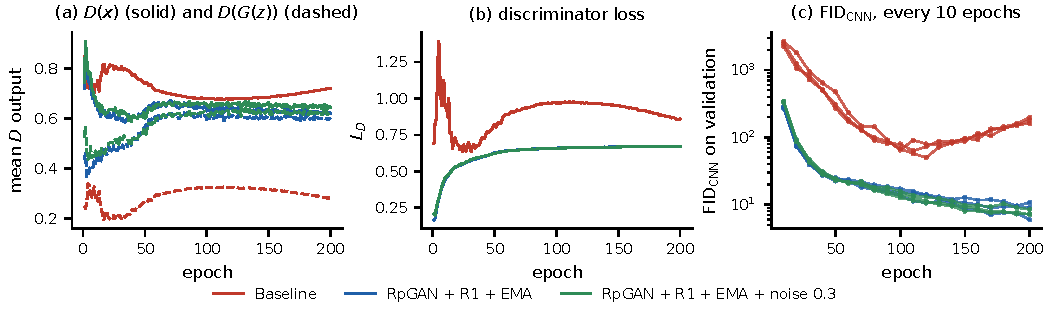
\includegraphics[width=\linewidth]{figs/supp/training_dynamics.pdf}
  \caption{Training of the common protocol (200 epochs, three seeds per configuration). (a) Mean output of $D$ on real (solid) and generated (dashed) images, mean over seeds. (b) Discriminator loss (BCE for the baseline, relativistic loss for the others). (c) \fcnn{} on the validation set, every 10 epochs, one line per seed (log scale).}
  \label{fig:supp-training}
\end{figure}

\subsection{The baseline drifts}
The reference baseline was evaluated every two epochs with both FIDs (Figure~\ref{fig:supp-drift}). \fcnn{} is lowest at epoch 106 (55.7) and then rises to 169 at epoch 200, while \finc{} keeps decreasing until epoch 200 (37.0). Between these two epochs, the share of ``1''s grows from 14\% to 25\% and the share of ``2''s falls from 6\% to 2\%: the generator draws its easy digits better and better and its hard digits more and more rarely. \fcnn{} sees the second effect, \finc{} mostly the first (Section~\ref{sec:fid}). This is the drift that the EMA cannot undo (Section~\ref{app:ema}).

\begin{figure}[H]
  \centering
  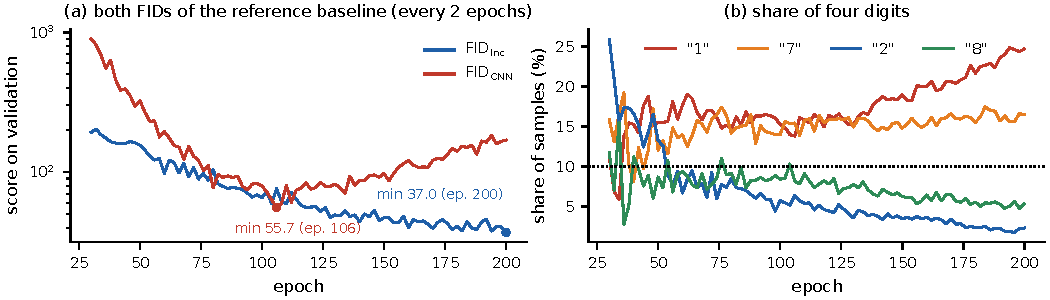
\includegraphics[width=\linewidth]{figs/supp/baseline_drift.pdf}
  \caption{Reference baseline (A100, seed 0), evaluated every two epochs on the validation set from epoch 30. (a) Both FIDs (log scale) and their minimum. (b) Share of four digits among 10,000 samples; the dotted line is 10\%.}
  \label{fig:supp-drift}
\end{figure}

\subsection{Choice of the loss and of $\gamma$}
Table~\ref{tab:supp-campaign} gives the campaign that selected the loss, scored with the classifier features used during training. The relativistic loss without penalty collapses; with R1 at $\gamma=1$ it divides \fcnn{} by four compared with the baseline and no seed collapses. Adding R2 (full R3GAN) gives no measurable gain, and R3GAN's recommended Adam setting ($\beta_1=0$) collapses with this architecture. Samples of these runs are shown in Figure~\ref{fig:supp-campaign}.

% Generated by regenerate_supplementary.py from results.csv and logs/ of the branch noe/training
\begin{table}[H]
\centering
\footnotesize
\setlength{\tabcolsep}{4pt}
\begin{tabular}{lrrrrrrr}
\toprule
Configuration & s0 & s1 & s2 & \fcnn{} & P & R & Digits (\%) \\
\midrule
Baseline (BCE) & 62.1 & 55.2 & \textit{c} (2770) & 58.7 $\pm$ 4.8 & 0.80 & 0.79 & 4--16 \\
RpGAN + R1, $\gamma=0.1$ & \textit{d} (2390 at ep.\ 20) & \textit{d} (2225 at ep.\ 20) & \textit{d} (2091 at ep.\ 20) & -- & -- & -- & -- \\
RpGAN + R1, $\gamma=1$ & 14.2 & 13.1 & 14.8 & 14.0 $\pm$ 0.9 & 0.72 & 0.80 & 8--13 \\
RpGAN + R1, $\gamma=10$ & 17.3 & 18.7 & 17.1 & 17.7 $\pm$ 0.9 & 0.67 & 0.79 & 7--13 \\
R3GAN (R1 + R2), $\gamma=1$ & 13.4 & 15.2 & 14.7 & 14.4 $\pm$ 0.9 & 0.70 & 0.80 & 8--13 \\
\midrule
\multicolumn{8}{l}{\textit{First series: 50 epochs, seed 0, no EMA}} \\
Baseline (BCE) & 188.0 &  &  &  & 0.64 & 0.32 & 5--17 \\
RpGAN, no penalty & \textit{c} (2619) &  &  &  & 0.00 & 0.00 & 0--100 \\
RpGAN + R1, $\gamma=1$ & 43.6 &  &  &  & 0.65 & 0.60 & 8--13 \\
R3GAN, $\gamma=1$ & 48.9 &  &  &  & 0.65 & 0.58 & 6--13 \\
R3GAN, $\gamma=1$, Adam $\beta=(0, 0.99)$ & \textit{c} (1540) &  &  &  & 0.46 & 0.00 & 0--34 \\
\bottomrule
\end{tabular}
\caption{Loss campaign (100 epochs, EMA 0.999, three seeds; scores against the 10,000 validation images, with the classifier features used during training). \textit{c}: collapsed run; \textit{d}: diverged run, stopped (last \fcnn{} printed in its log). P, R: classifier precision and recall ($k=3$); Digits: range of the share of each digit (\%).}
\label{tab:supp-campaign}
\end{table}


% ==========================================================================================
\section{Generated Examples}
\label{app:examples}

\subsection{Same latent vectors through each configuration}
Figure~\ref{fig:supp-samez} feeds the same 100 latent vectors to the generators of seed 1. The raw and averaged generators of the RpGAN run (b, c) draw the same digit for almost every $z$: the EMA does not change \emph{what} is drawn but cleans the strokes. The baseline (a) draws different digits for the same $z$ and many ``1''s. Instance noise (d) gives a different but equally clean generator.

\begin{figure}[H]
  \centering
  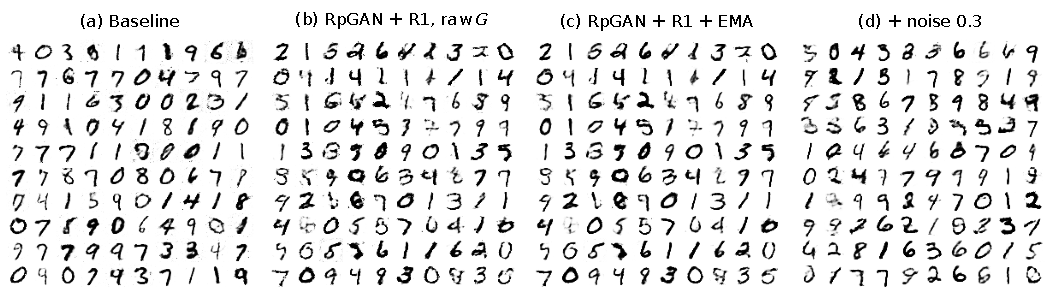
\includegraphics[width=\linewidth]{figs/supp/examples_same_z.pdf}
  \caption{The same 100 latent vectors through four generators of seed 1 of the common protocol (epoch 200). (a) Baseline. (b) RpGAN + R1, raw generator. (c) Same run, averaged generator. (d) RpGAN + R1 + EMA + instance noise 0.3, averaged generator.}
  \label{fig:supp-samez}
\end{figure}

\begin{figure}[H]
  \centering
  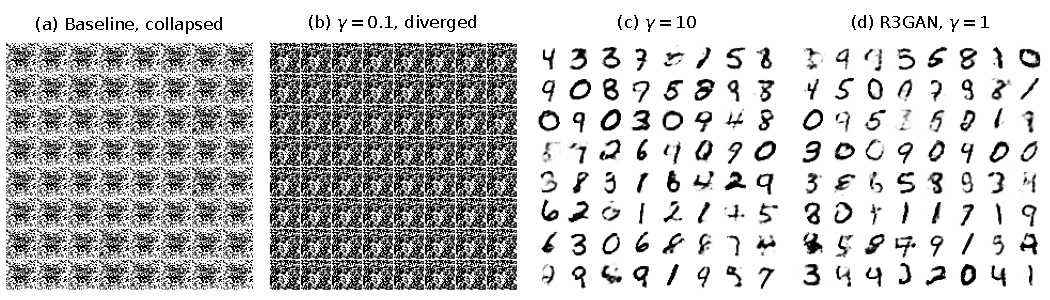
\includegraphics[width=\linewidth]{figs/supp/examples_campaign.pdf}
  \caption{Loss campaign (100 epochs), same latent vectors. (a) Collapsed baseline run (seed 2): $D$ saturated at epoch 7 and $G$ outputs noise. (b) RpGAN + R1 with $\gamma=0.1$ (seed 0): diverged, stopped at epoch 28. (c) $\gamma=10$ (seed 0): readable digits, with more broken strokes. (d) R3GAN with $\gamma=1$ (seed 0).}
  \label{fig:supp-campaign}
\end{figure}

\subsection{Samples sorted by digit}
Figure~\ref{fig:supp-bydigit} sorts 10,000 samples of each generator by the digit our classifier predicts. The baseline draws a ``1'' in 25\% of its images and a ``2'' in 1.2\%, and its rare digits (2, 3, 5, 8) are its worst drawn ones. RpGAN + R1 + EMA draws every digit 8--12\% of the time, and its ``2''s are mostly readable.

\begin{figure}[H]
  \centering
  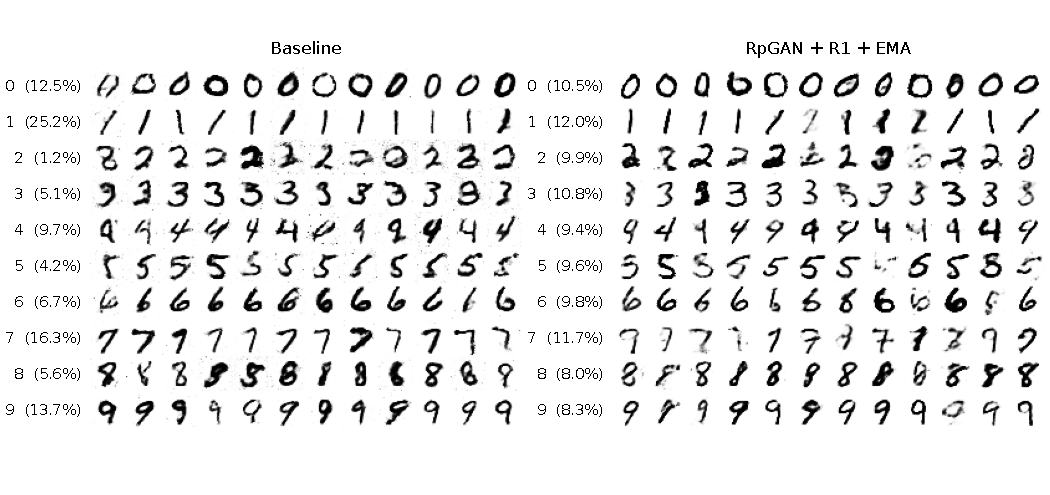
\includegraphics[width=\linewidth]{figs/supp/examples_by_digit.pdf}
  \caption{The first 12 images classified as each digit among 10,000 samples (seed 1, common protocol). The number next to each digit is its share among the 10,000 samples.}
  \label{fig:supp-bydigit}
\end{figure}

\subsection{What OBRS rejects in the submitted model}
Figure~\ref{fig:supp-obrs} uses the submitted generator and the recalibrated $D$, with the threshold of OBRS at $K=3$. The proposals with the lowest acceptance probability are malformed or ambiguous digits, often ``2''s, ``3''s, ``0''s and ``8''s; 9.1\% of proposals have a score above the threshold and are always kept. The acceptance probability is almost the same for every digit (0.31--0.40): the recalibrated filter removes badly drawn images within each digit and barely changes the digit balance, which is why \fcnn{} stays at 10 (Table~\ref{tab:supp-rejection}).

\begin{figure}[H]
  \centering
  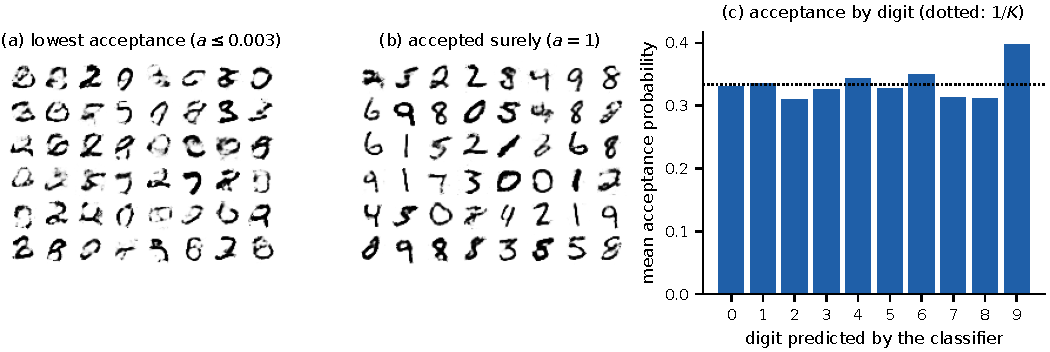
\includegraphics[width=\linewidth]{figs/supp/obrs_kept_rejected.pdf}
  \caption{Submitted model (RpGAN + R1 + EMA, OBRS with $K=3$ and the recalibrated $D$ of \texttt{checkpoints/}), 50,000 proposals. (a) The 48 proposals with the lowest acceptance probability. (b) 48 proposals accepted with probability 1. (c) Mean acceptance probability per predicted digit.}
  \label{fig:supp-obrs}
\end{figure}

% ==========================================================================================
\section{Full Results}
\label{app:results}

\subsection{Common protocol: every run}
Table~\ref{tab:supp-common} gives the score of every seed behind Tables~\ref{tab:data}, \ref{tab:loss-ema} and~\ref{tab:results} of the report. The two blocks were trained on different machines, so only rows within one block are compared. The baseline with noise collapsed for 2 of its 5 seeds; no RpGAN + R1 run collapsed.

% Generated by regenerate_supplementary.py from data/comparison_local.csv and data/juliet2_test.csv
\begin{table}[H]
\centering
\footnotesize
\setlength{\tabcolsep}{4pt}
\begin{tabular}{lrrrrrrrrrr}
\toprule
Configuration & s0 & s1 & s2 & s3 & s4 & \finc{} & P & R & \fcnn{} & Kept \\
\midrule
\multicolumn{11}{l}{\textit{Trained on the Apple M3}} \\
Baseline & 39.9 & 37.4 & 38.7 &  &  & 38.7 $\pm$ 1.2 & 0.47 & 0.51 & 181.8 & 100\% \\
Baseline + DRS & 33.9 & 35.2 & 34.0 &  &  & 34.4 $\pm$ 0.7 & 0.51 & 0.49 & 154.0 & 30\% \\
RpGAN + R1 + EMA & 23.6 & 21.2 & 21.7 &  &  & 22.1 $\pm$ 1.3 & 0.59 & 0.59 & 9.9 & 100\% \\
RpGAN + R1 + EMA + DRS & 23.2 & 21.9 & 21.0 &  &  & 22.0 $\pm$ 1.1 & 0.59 & 0.58 & 14.2 & 43\% \\
RpGAN + R1 + EMA + noise 0.3 & 22.1 & 21.1 & 21.1 &  &  & 21.4 $\pm$ 0.6 & 0.60 & 0.61 & 9.0 & 100\% \\
RpGAN + R1 + EMA + noise 0.3 + DRS & 22.5 & 22.7 & 20.6 &  &  & 21.9 $\pm$ 1.1 & 0.60 & 0.60 & 13.9 & 42\% \\
RpGAN + R1, raw $G$ & 38.8 & 37.6 & 36.7 &  &  & 37.7 $\pm$ 1.0 & 0.47 & 0.47 & 19.7 & 100\% \\
RpGAN + R1, raw $G$ + DRS & 39.4 & 38.4 & 36.1 &  &  & 38.0 $\pm$ 1.7 & 0.46 & 0.47 & 21.6 & 43\% \\
RpGAN + R1 + noise 0.3, raw $G$ & 36.6 & 35.5 & 35.3 &  &  & 35.8 $\pm$ 0.7 & 0.48 & 0.50 & 18.3 & 100\% \\
RpGAN + R1 + noise 0.3, raw $G$ + DRS & 37.3 & 36.5 & 34.7 &  &  & 36.2 $\pm$ 1.3 & 0.48 & 0.51 & 19.0 & 42\% \\
\midrule
\multicolumn{11}{l}{\textit{Trained on the A100}} \\
Baseline, raw $G$ & 37.0 & 37.7 & 35.2 &  &  & 36.6 $\pm$ 1.3 & 0.48 & 0.49 & 169.8 & 100\% \\
Baseline, raw $G$ + DRS & 31.4 & 30.6 & 31.9 &  &  & 31.3 $\pm$ 0.7 & 0.54 & 0.48 & 159.8 & 30\% \\
Baseline + EMA & 30.1 & 29.8 & 30.0 &  &  & 30.0 $\pm$ 0.2 & 0.56 & 0.54 & 181.5 & 100\% \\
Baseline + EMA + DRS & 24.9 & 23.8 & 25.8 &  &  & 24.8 $\pm$ 1.0 & 0.62 & 0.53 & 166.7 & 31\% \\
Baseline + noise 0.3, raw $G$ & \textit{c} & 45.2 & 41.8 & \textit{c} & 40.5 & 42.5 $\pm$ 2.4 & 0.44 & 0.48 & 183.8 & 100\% \\
Baseline + noise 0.3, raw $G$ + DRS & \textit{c} & 39.1 & 38.5 & \textit{c} & 35.8 & 37.8 $\pm$ 1.8 & 0.48 & 0.48 & 162.1 & 31\% \\
Baseline + noise 0.3 + EMA & \textit{c} & 31.5 & 28.8 & \textit{c} & 29.9 & 30.1 $\pm$ 1.3 & 0.56 & 0.54 & 186.7 & 100\% \\
Baseline + noise 0.3 + EMA + DRS & \textit{c} & 26.3 & 24.7 & \textit{c} & 25.0 & 25.3 $\pm$ 0.8 & 0.62 & 0.53 & 150.7 & 31\% \\
\bottomrule
\end{tabular}
\caption{Every run of the common protocol (200 epochs, last checkpoint, test set). Columns s0--s4: \finc{} of each seed; \textit{c}: collapsed run, excluded from the means. P, R: VGG precision and recall; Kept: share of proposals kept by DRS. ``Raw $G$'' is the non-averaged generator of the same run. Rows of one block share their runs, so their differences are paired.}
\label{tab:supp-common}
\end{table}


\subsection{Digit balance}
Table~\ref{tab:supp-digits} gives the share of each digit. The EMA does not change the balance of the baseline (``2'': 1.6\% for the baseline and for the averaged baseline); the relativistic loss does. DRS with $D$ as trained slightly reduces the share of ``1''s of the baseline (25.1\% to 22.0\%) but leaves the ``2''s at 1.8\%.

% Generated by regenerate_supplementary.py from data/comparison_local.csv and data/juliet2_test.csv
\begin{table}[H]
\centering
\footnotesize
\setlength{\tabcolsep}{4pt}
\begin{tabular}{lrrrrrrrrrr}
\toprule
Model & 0 & 1 & 2 & 3 & 4 & 5 & 6 & 7 & 8 & 9 \\
\midrule
Real test set & 9.8 & 11.3 & 10.3 & 10.1 & 9.8 & 8.9 & 9.6 & 10.3 & 9.7 & 10.1 \\
Baseline & 12.5 & 25.1 & 1.6 & 5.7 & 8.9 & 4.7 & 7.9 & 16.0 & 5.4 & 12.3 \\
Baseline + DRS & 11.2 & 22.0 & 1.8 & 5.8 & 9.7 & 4.8 & 9.3 & 15.9 & 5.8 & 13.8 \\
RpGAN + R1 + EMA & 10.5 & 11.8 & 9.8 & 10.5 & 9.9 & 9.8 & 9.5 & 12.0 & 8.0 & 8.2 \\
RpGAN + R1 + EMA + DRS & 10.8 & 11.1 & 9.9 & 10.3 & 10.0 & 9.2 & 9.9 & 12.3 & 7.6 & 8.9 \\
RpGAN + R1 + EMA + noise 0.3 & 10.4 & 11.8 & 9.5 & 10.5 & 10.0 & 9.6 & 9.8 & 11.8 & 8.4 & 8.3 \\
Baseline + EMA & 12.0 & 24.7 & 1.6 & 6.2 & 8.8 & 4.6 & 7.1 & 16.2 & 5.3 & 13.4 \\
RpGAN + R1, raw $G$ & 10.1 & 11.6 & 10.4 & 11.0 & 10.3 & 9.7 & 9.4 & 11.8 & 8.1 & 7.5 \\
\bottomrule
\end{tabular}
\caption{Share of each digit (\%) among 10,000 samples, as predicted by the classifier (mean over the non-collapsed seeds).}
\label{tab:supp-digits}
\end{table}


\subsection{Per-digit FID}
Table~\ref{tab:supp-perdigit} gives the per-digit \finc{} behind Figure~\ref{fig:perdigit} of the report. For every model, ``2'' is the worst digit. At fixed digit, the relativistic loss lowers the score of 7 digits out of 10, mostly the hard ones (``2'': 113 to 80; ``5'': 83 to 63), and raises it for ``0'', ``1'' and ``7'', while the global score barely moves (38.7 to 37.7). The EMA then lowers all ten.

% Generated by regenerate_supplementary.py from data/kid_perclass_all.csv
\begin{table}[H]
\centering
\footnotesize
\setlength{\tabcolsep}{4pt}
\begin{tabular}{lrrrrrrrrrrrr}
\toprule
Model & 0 & 1 & 2 & 3 & 4 & 5 & 6 & 7 & 8 & 9 & Mean & All \\
\midrule
Real (validation) & 7.7 & 7.7 & 10 & 6.5 & 8.8 & 9.1 & 9.1 & 10 & 8.1 & 7.8 & 8.5 & 1.5 \\
Baseline & 49 & 37 & 113 & 71 & 59 & 83 & 56 & 51 & 70 & 48 & 63.6 & 38.7 \\
Baseline + DRS & 45 & 31 & 110 & 62 & 55 & 74 & 47 & 45 & 59 & 42 & 57.0 & 34.4 \\
RpGAN + R1, raw $G$ & 50 & 52 & 80 & 53 & 51 & 63 & 54 & 56 & 55 & 40 & 55.4 & 37.7 \\
RpGAN + R1 + EMA & 27 & 34 & 58 & 41 & 35 & 46 & 33 & 34 & 39 & 25 & 37.3 & 22.1 \\
RpGAN + R1 + EMA + DRS & 27 & 34 & 59 & 41 & 36 & 45 & 33 & 35 & 38 & 25 & 37.3 & 22.0 \\
RpGAN + R1 + EMA + noise 0.3 & 28 & 35 & 58 & 37 & 36 & 44 & 33 & 35 & 39 & 25 & 37.0 & 21.4 \\
\bottomrule
\end{tabular}
\caption{Per-digit \finc{}: the classifier assigns each generated image to a digit, and 1,000 images of each digit are compared with real test images of the same digit (mean over three seeds). Mean: unweighted mean over digits; All: global \finc{} of the same images.}
\label{tab:supp-perdigit}
\end{table}


\subsection{Data lever: every run}
Table~\ref{tab:supp-data} gives every run of the data lever. Every configuration trained with five seeds or more has collapsed runs, from 2 of 5 (selection at 95\% and 90\%) to 4 of 8 (selection at 50\%, annealed noise at $\sigma_0=0.1$). The paired rerun with 8 seeds gives 3 collapses without noise and 1 with noise ($p=0.57$, Fisher's exact test).

% Generated by regenerate_supplementary.py from data/nico_data_test.csv and data/noise_rerun_test.csv
\begin{table}[H]
\centering
\footnotesize
\setlength{\tabcolsep}{4pt}
\begin{tabular}{lrrrrrrrrrrrr}
\toprule
Configuration & s0 & s1 & s2 & s3 & s4 & s5 & s6 & s7 & \finc{} & P & R & \fcnn{} \\
\midrule
Reference (no selection) & 36.8 & 34.4 & 35.0 & 35.5 & \textit{c} & \textit{c} & \textit{c} & 35.1 & 35.4 $\pm$ 0.9 & 0.51 & 0.52 & 220.5 \\
Selection 95\% & \textit{c} & 36.8 & 41.3 & \textit{c} & 36.6 &  &  &  & 38.2 $\pm$ 2.7 & 0.49 & 0.48 & 211.3 \\
Selection 90\% & \textit{c} & 38.9 & 36.3 & \textit{c} & 32.3 &  &  &  & 35.8 $\pm$ 3.3 & 0.53 & 0.49 & 246.0 \\
Selection 75\% & 37.9 & 45.2 & 39.3 &  &  &  &  &  & 40.8 $\pm$ 3.9 & 0.54 & 0.40 & 446.8 \\
Selection 50\% & 47.2 & \textit{c} & \textit{c} & \textit{c} & 44.5 & 51.5 & 48.1 & \textit{c} & 47.8 $\pm$ 2.9 & 0.56 & 0.32 & 719.3 \\
Selection 50\%, one Gaussian for all digits & 45.1 & 42.3 & 43.6 &  &  &  &  &  & 43.7 $\pm$ 1.4 & 0.49 & 0.37 & 521.2 \\
Selection 50\%, Gaussian on pixels & 49.2 & \textit{c} & \textit{c} &  &  &  &  &  & 49.2 & 0.53 & 0.26 & 833.9 \\
Noise $\sigma_0=0.1$, annealed & \textit{c} & 37.6 & \textit{c} & 32.8 & 37.7 & \textit{c} & 34.0 & \textit{c} & 35.5 $\pm$ 2.5 & 0.52 & 0.52 & 227.7 \\
Noise $\sigma=0.1$, constant & 34.0 & \textit{c} & \textit{c} &  &  &  &  &  & 34.0 & 0.53 & 0.55 & 195.9 \\
Noise $\sigma_0=0.3$, annealed & 37.4 & 35.2 & 38.3 &  &  &  &  &  & 37.0 $\pm$ 1.6 & 0.51 & 0.52 & 223.5 \\
Selection 50\% + noise 0.1 & 44.0 & 44.5 & 53.5 &  &  &  &  &  & 47.4 $\pm$ 5.4 & 0.57 & 0.31 & 718.1 \\
Reference, rerun (100 epochs) & 56.7 & 53.4 & 59.4 & 53.4 & \textit{c} & \textit{c} & \textit{c} & 53.9 & 55.3 $\pm$ 2.6 & 0.29 & 0.42 & 77.0 \\
Noise $\sigma_0=0.3$, rerun (100 epochs) & 56.0 & 51.4 & 58.9 & \textit{c} & 54.4 & 59.2 & 50.6 & 49.5 & 54.3 $\pm$ 3.9 & 0.29 & 0.40 & 67.2 \\
\bottomrule
\end{tabular}
\caption{Every run of the data lever (data protocol: 60,000 images, 120,000 updates, no EMA; test set). Columns s0--s7: \finc{} of each seed; \textit{c}: collapsed run, excluded from the means. The two reruns use 8 paired seeds and 100 epochs.}
\label{tab:supp-data}
\end{table}


\subsection{Rejection: every variant}
Table~\ref{tab:supp-rejection} completes Table~\ref{tab:rejection} of the report with OBRS and DRS for both models, with $D$ as trained and recalibrated. Figure~\ref{fig:supp-scores} shows why $D$ as trained helps the baseline but not the final model: the scores of real and generated images overlap almost completely for the averaged generator, which $D$ has never seen.

% Generated by regenerate_supplementary.py from data/drs_recalib_test.csv
\begin{table}[H]
\centering
\footnotesize
\setlength{\tabcolsep}{4pt}
\begin{tabular}{lrrrrrrrrrr}
\toprule
Rejection & s0 & s1 & s2 & \finc{} & P & R & \fcnn{} & Kept & AUC & Time (s) \\
\midrule
\multicolumn{10}{l}{\textit{Baseline}} \\
none & 39.5 & 37.8 & 38.7 & 38.7 $\pm$ 0.9 & 0.47 & 0.50 & 182.7 & 100\% & 0.75 & 0.03 \\
DRS & 33.6 & 35.1 & 34.1 & 34.3 $\pm$ 0.8 & 0.51 & 0.50 & 154.1 & 30\% & 0.75 & 0.14 \\
OBRS $K=3$ & 33.0 & 34.8 & 33.4 & 33.8 $\pm$ 0.9 & 0.51 & 0.50 & 144.6 & 33\% & 0.75 & 0.17 \\
DRS, recalibrated $D$ & 35.6 & 36.9 & 36.4 & 36.3 $\pm$ 0.7 & 0.46 & 0.51 & 103.4 & 32\% & 0.83 & 0.09 \\
OBRS $K=3$, recalibrated $D$ & 35.6 & 37.2 & 35.5 & 36.1 $\pm$ 0.9 & 0.46 & 0.52 & 82.9 & 33\% & 0.83 & 0.16 \\
\multicolumn{10}{l}{\textit{RpGAN + R1 + EMA}} \\
none & 23.6 & 21.2 & 21.3 & 22.0 $\pm$ 1.4 & 0.59 & 0.59 & 9.9 & 100\% & 0.57 & 0.02 \\
DRS & 23.3 & 22.0 & 21.2 & 22.1 $\pm$ 1.1 & 0.59 & 0.59 & 14.4 & 42\% & 0.57 & 0.07 \\
OBRS $K=3$ & 22.9 & 21.9 & 21.2 & 22.0 $\pm$ 0.9 & 0.59 & 0.59 & 13.2 & 45\% & 0.57 & 0.15 \\
DRS, recalibrated $D$ & 21.5 & 19.9 & 19.2 & 20.2 $\pm$ 1.2 & 0.62 & 0.59 & 10.0 & 32\% & 0.77 & 0.09 \\
OBRS $K=3$, recalibrated $D$ & 20.7 & 19.4 & 19.2 & 19.7 $\pm$ 0.8 & 0.62 & 0.59 & 10.2 & 33\% & 0.77 & 0.16 \\
\bottomrule
\end{tabular}
\caption{Every rejection variant on the three seeds of each model (common protocol, test set, mean of two draws of 10,000 images per seed). AUC: how well the score separates real validation images from generated ones; Time: seconds to draw 10,000 images on an A100.}
\label{tab:supp-rejection}
\end{table}


\begin{figure}[H]
  \centering
  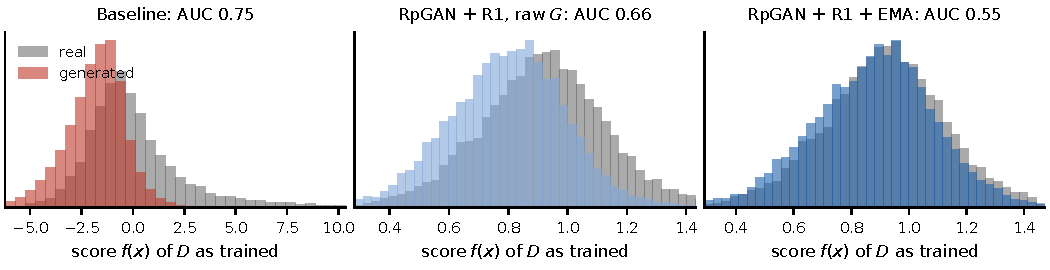
\includegraphics[width=\linewidth]{figs/supp/d_scores.pdf}
  \caption{Histograms of the score $f$ of $D$ as trained on real and generated images (seed 1). The AUC is computed from the histograms, on other images than in Table~\ref{tab:supp-rejection}, hence the small differences. The averaged generator (right) is scored by the $D$ trained against the raw generator.}
  \label{fig:supp-scores}
\end{figure}

\subsection{Budget of the rejection methods}
Before the common protocol, the inference lever was explored on an early baseline with the classifier features (Figure~\ref{fig:supp-budget}a and Table~\ref{tab:supp-budget}). OBRS is better than DRS for every budget from $K=2$ to $K=10$, and both stop improving beyond $K=10$, while the cost grows linearly with $K$. Truncating the latent vector, a common trick of large GANs, does not help: at $\psi=3$ it scores 95.3 against 97.6 without truncation, within the noise of the draws, and for smaller $\psi$ it removes whole digits (at $\psi=0.5$, 95\% of the samples are ``9''s). On the reference baseline (Figure~\ref{fig:supp-budget}b), DRS improves \finc{} from 36.7 to about 31.5 at every percentile from 80 to 99, and the KeepTraining step of \cite{azadi2019} (fine-tuning $D$ before filtering) removes most of this gain. We therefore used percentile 80 without KeepTraining, and $K=3$ for OBRS.

\begin{figure}[H]
  \centering
  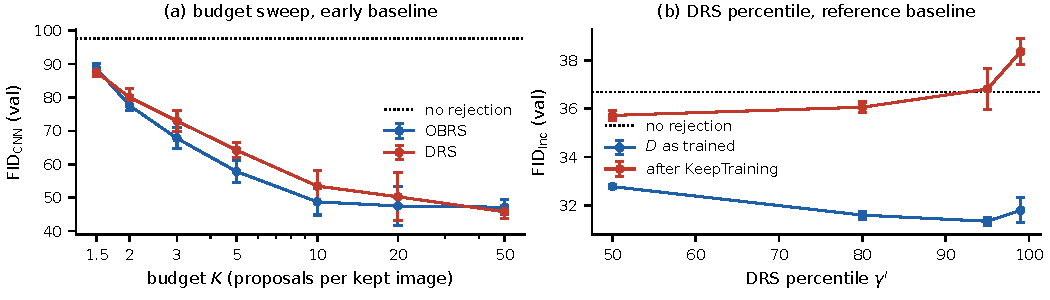
\includegraphics[width=\linewidth]{figs/supp/budget_sweep.pdf}
  \caption{(a) \fcnn{} of OBRS and DRS as a function of the budget $K$ (early baseline, three draws). (b) \finc{} of DRS as a function of the percentile $\gamma'$, with $D$ as trained or after KeepTraining (reference baseline, epoch 200, three draws). Both against the validation set.}
  \label{fig:supp-budget}
\end{figure}

% Generated by regenerate_supplementary.py from results/results.csv of the branch noe/training
\begin{table}[H]
\centering
\footnotesize
\setlength{\tabcolsep}{4pt}
\begin{tabular}{llrrrrr}
\toprule
Method & Value & \fcnn{} & P & R & Kept & Time (s) \\
\midrule
OBRS, budget $K$ & 1.5 & 88.7 $\pm$ 1.6 & 0.85 & 0.74 & 67\% & 2.8 \\
 & 2 & 77.5 $\pm$ 1.5 & 0.85 & 0.74 & 50\% & 3.2 \\
 & 3 & 67.8 $\pm$ 3.1 & 0.85 & 0.75 & 33\% & 3.3 \\
 & 5 & 57.8 $\pm$ 3.3 & 0.85 & 0.75 & 20\% & 4.1 \\
 & 10 & 48.8 $\pm$ 3.9 & 0.85 & 0.75 & 10\% & 6.1 \\
 & 20 & 47.5 $\pm$ 5.8 & 0.85 & 0.74 & 5\% & 10.3 \\
 & 50 & 47.1 $\pm$ 2.2 & 0.85 & 0.74 & 2\% & 20.1 \\
\midrule
DRS, budget $K$ & 1.5 & 87.6 $\pm$ 1.3 & 0.85 & 0.75 & 67\% & 2.9 \\
 & 2 & 80.0 $\pm$ 2.8 & 0.85 & 0.75 & 50\% & 2.9 \\
 & 3 & 73.0 $\pm$ 3.0 & 0.85 & 0.75 & 34\% & 3.3 \\
 & 5 & 64.2 $\pm$ 2.2 & 0.85 & 0.75 & 20\% & 4.1 \\
 & 10 & 53.5 $\pm$ 4.7 & 0.85 & 0.75 & 10\% & 6.1 \\
 & 20 & 50.3 $\pm$ 7.2 & 0.85 & 0.74 & 5\% & 9.8 \\
 & 50 & 45.8 $\pm$ 1.9 & 0.86 & 0.74 & 2\% & 22.4 \\
\midrule
Truncation, $\psi$ & 0.5 & 1916.8 $\pm$ 11.3 & 0.97 & 0.05 & 100\% & 0.2 \\
 & 1 & 598.1 $\pm$ 7.9 & 0.91 & 0.35 & 100\% & 0.2 \\
 & 1.5 & 231.6 $\pm$ 3.2 & 0.88 & 0.60 & 100\% & 0.3 \\
 & 2 & 133.8 $\pm$ 1.6 & 0.86 & 0.70 & 100\% & 0.3 \\
 & 2.5 & 104.4 $\pm$ 1.2 & 0.84 & 0.73 & 100\% & 0.2 \\
 & 3 & 95.3 $\pm$ 1.2 & 0.84 & 0.74 & 100\% & 0.2 \\
\midrule
No rejection &  & 97.6 $\pm$ 4.4 & 0.83 & 0.74 & 100\% &  \\
\bottomrule
\end{tabular}
\caption{Sampling methods on an early baseline (\texttt{checkpoints/G.pth} at the start of the project, provided loss), three draws of 10,000 images against the validation set, classifier features. Truncation draws each coordinate of $z$ from a standard normal truncated to $[-\psi,\psi]$. Kept: share of proposals kept; Time: seconds on an Apple M3.}
\label{tab:supp-budget}
\end{table}


\subsection{Sensitivity of both FIDs}
Table~\ref{tab:supp-sensitivity} gives every condition of Figure~\ref{fig:fid} of the report, and four more: blur, chimera digits (the average of two images of different digits), erased squares and thicker strokes. Light pixel noise moves \finc{} much more than \fcnn{} (noise $\sigma=0.1$ on every image: 132 against 25), damage to the strokes moves \fcnn{} more (blur on every image: 62 against 566), and removing or unbalancing digits moves almost only \fcnn{}.

% Generated by regenerate_supplementary.py from data/sensitivity_10k.csv
\begin{table}[H]
\centering
\footnotesize
\setlength{\tabcolsep}{4pt}
\begin{tabular}{llrrr}
\toprule
Damage & Level & \finc{} & \fcnn{} & KID \\
\midrule
Real training vs real test images &  & 1.5 & 2.7 & 0.11 \\
\midrule
Baseline GAN &  & 39.9 & 162.3 & 30.25 \\
Baseline, resampled to equal digit shares &  & 46.2 & 31.6 & 40.25 \\
RpGAN + R1 + EMA &  & 23.6 & 12.5 & 17.11 \\
\midrule
Gaussian pixel noise, $\sigma=0.1$ & 10\% of images & 8.4 & 3.1 & 2.09 \\
Gaussian pixel noise, $\sigma=0.1$ & 25\% of images & 22.7 & 4.3 & 11.88 \\
Gaussian pixel noise, $\sigma=0.1$ & 50\% of images & 52.1 & 8.5 & 46.11 \\
Gaussian pixel noise, $\sigma=0.1$ & 100\% of images & 132.0 & 25.2 & 182.77 \\
\midrule
Gaussian pixel noise, $\sigma=0.3$ & 10\% of images & 15.2 & 5.6 & 3.59 \\
Gaussian pixel noise, $\sigma=0.3$ & 25\% of images & 41.4 & 17.9 & 20.72 \\
Gaussian pixel noise, $\sigma=0.3$ & 50\% of images & 92.0 & 61.7 & 80.21 \\
Gaussian pixel noise, $\sigma=0.3$ & 100\% of images & 230.3 & 269.2 & 318.51 \\
\midrule
Gaussian blur, $\sigma=1$ & 10\% of images & 3.2 & 9.5 & 0.72 \\
Gaussian blur, $\sigma=1$ & 25\% of images & 8.3 & 38.8 & 3.73 \\
Gaussian blur, $\sigma=1$ & 50\% of images & 20.3 & 135.4 & 14.14 \\
Gaussian blur, $\sigma=1$ & 100\% of images & 62.2 & 566.2 & 56.16 \\
\midrule
Average with an image of another digit & 10\% of images & 3.1 & 7.8 & 0.59 \\
Average with an image of another digit & 25\% of images & 7.5 & 31.5 & 2.95 \\
Average with an image of another digit & 50\% of images & 18.3 & 115.8 & 11.21 \\
Average with an image of another digit & 100\% of images & 53.5 & 541.0 & 43.97 \\
\midrule
Erase a random $10\times10$ square & 10\% of images & 3.0 & 6.6 & 0.66 \\
Erase a random $10\times10$ square & 25\% of images & 7.1 & 22.3 & 3.26 \\
Erase a random $10\times10$ square & 50\% of images & 17.7 & 74.4 & 12.54 \\
Erase a random $10\times10$ square & 100\% of images & 52.0 & 280.4 & 49.82 \\
\midrule
Thicker strokes ($3\times3$ dilation) & 10\% of images & 2.9 & 4.6 & 0.63 \\
Thicker strokes ($3\times3$ dilation) & 25\% of images & 8.1 & 13.9 & 3.80 \\
Thicker strokes ($3\times3$ dilation) & 50\% of images & 21.6 & 43.8 & 15.48 \\
Thicker strokes ($3\times3$ dilation) & 100\% of images & 69.2 & 165.3 & 63.05 \\
\midrule
Digits removed & 1 digit & 2.4 & 39.5 & 0.49 \\
Digits removed & 2 digits & 4.2 & 114.6 & 1.43 \\
Digits removed & 5 digits & 10.9 & 342.9 & 4.87 \\
Digit imbalance & 30\% of ``1'' & 6.8 & 84.8 & 5.35 \\
Digit imbalance & 20\% of ``1'' & 2.8 & 23.5 & 1.36 \\
Digit imbalance & baseline's shares & 7.4 & 123.6 & 6.57 \\
\bottomrule
\end{tabular}
\caption{Both FIDs (and the Inception KID $\times 1000$) on deliberately damaged real test images, against the real test set (10,000 images, mean of three draws). The damage is applied to the indicated share of the images; ``digits removed'' replaces the images of the removed digits by images of the remaining ones.}
\label{tab:supp-sensitivity}
\end{table}


% ==========================================================================================
\section{Reproducibility}
\label{app:repro}

\subsection{Settings}
Table~\ref{tab:supp-hyper} lists the settings of the two main configurations; they are read from the configuration files saved with each run.

% Generated by regenerate_supplementary.py from runs/cmploc_*/config.yaml of the branch noe/training
\begin{table}[H]
\centering
\footnotesize
\setlength{\tabcolsep}{4pt}
\begin{tabular}{p{3.2cm}p{6.2cm}p{4.6cm}}
\toprule
Setting & Baseline & RpGAN + R1 + EMA \\
\midrule
Optimizer (G and D) & Adam, lr 0.0002, $\beta=(0.9, 0.999)$ & same \\
Batch size, epochs, updates & 100, 200, 100,000 & same \\
Loss & BCE (\texttt{nn.BCELoss} on $\sigma(f)$) & RpGAN, R1 $\gamma=1$, R2 $\gamma=0$ \\
EMA of $G$ & none & decay 0.999 \\
Evaluation during training & \fcnn{}, every 10 epochs, 10,000 images & same \\
Weights evaluated & epoch 200 (no choice of epoch) & same \\
DRS & percentile 80, $\epsilon=10^{-6}$, 10,000 burn-in proposals & same \\
OBRS & $K=3$, threshold fitted on 50,000 proposals & same \\
Recalibration & last layer of $D$, logistic regression, 10k real val vs 10k generated & same \\
Software & Python 3.12.6, PyTorch 2.6.0 & same \\
\bottomrule
\end{tabular}
\caption{Settings of the common protocol. The data-lever runs differ only by their data (60,000 images, 120 epochs).}
\label{tab:supp-hyper}
\end{table}


\subsection{Code and runs}
The code is in the group repository (\texttt{github.com/Master-IASD/masteriasd-datalab-project-a2-group-3}). \texttt{train.py} trains one configuration from a YAML file (\texttt{configs/}); the loss, R1, R2, the EMA and instance noise are optional sections of this file, and without them the training is exactly the provided one. Each run saves its configuration, git commit, environment, per-epoch metrics (\texttt{metrics.jsonl}), the averaged and raw generators and its discriminator in \texttt{runs/<name>/}. \texttt{evaluate.py} scores a run with any sampling method of \texttt{sampling.py} (plain, truncation, DRS, OBRS) against the train, validation or test split, and \texttt{generate.py} draws the 10,000 submitted images with the method written in \texttt{checkpoints/sampling.yaml}. The same configuration on the same machine gives bit-identical weights, including after resuming from a checkpoint. A run of 200 epochs takes 1.5 to 2.5 hours on the M3 laptop (27 to 43 seconds per epoch).

\subsection{Regenerating the report}
\texttt{regenerate\_figures.py} copies the figures and result files of the report from the repository and recomputes every mean, standard deviation, collapse count and $p$-value of the main text. \texttt{regenerate\_supplementary.py} draws every figure and table of this supplementary material from the result files, the training logs and the trained generators; samples are drawn with fixed seeds.

\end{document}
